\documentclass[12pt,a4paper]{article}

\usepackage[utf8]{inputenc}
\usepackage[T1]{fontenc}
\usepackage[brazil]{babel}
\usepackage{geometry}
\usepackage{graphicx}
\usepackage{listings}
\usepackage{xcolor}
\usepackage{hyperref}
\usepackage{booktabs}
\usepackage{float}
\usepackage{amsmath}

\geometry{top=2cm, bottom=2cm, left=2.5cm, right=2.5cm}

\hypersetup{
    colorlinks=true,
    linkcolor=blue,
    urlcolor=blue
}

\lstset{
    basicstyle=\ttfamily\small,
    keywordstyle=\color{blue},
    commentstyle=\color{gray},
    language=C,
    frame=single,
    breaklines=true,
    numbers=left,
    numberstyle=\tiny
}

\title{
    \textbf{Sistemas Distribuídos -- CEFET-MG}\\
    \large Trabalho Prático 1: IPC, Threads e Sincronização\\
    2026/1
}
\author{Ester Morais Neves \and Laura Pianetti Veloso}
\date{\today}

% -------------------------------------------------------
\begin{document}
\maketitle
\thispagestyle{empty}

\textbf{Código-fonte:} \url{https://github.com/estermorais/Sistemas-Distribuidos/tree/main/TP1}

% -------------------------------------------------------
\section{Produtor-Consumidor com Pipes}

\subsection{Decisões de Projeto}

O programa utiliza um \emph{anonymous pipe} criado com \texttt{pipe(fd)} antes
do \texttt{fork()}, de forma que pai e filho herdem os dois descritores.
O processo \textbf{pai} assume o papel de produtor (usa \texttt{fd[1]}, write end)
e o processo \textbf{filho} assume o papel de consumidor (usa \texttt{fd[0]}, read
end). Cada processo fecha imediatamente o descritor que não utiliza, evitando
que o pipe permaneça aberto inadvertidamente.

\paragraph{Serialização das mensagens.}
Conforme recomendado pelo enunciado, cada número é convertido para uma string
de tamanho fixo de 20 bytes com \texttt{snprintf} + \texttt{memset}.
Isso garante que cada \texttt{read} recupere exatamente uma mensagem,
eliminando o risco de leituras parciais, problema comum ao tratar pipes como
fluxos de bytes sem delimitadores.

\paragraph{Geração de números.}
O produtor gera a sequência $N_i = N_{i-1} + \Delta$, com $N_0 = 1$ e
$\Delta \in [1, 100]$ escolhido aleatoriamente a cada iteração via
\texttt{rand()}.

\paragraph{Terminação.}
Após enviar a quantidade solicitada de números, o produtor envia o valor~$0$
como sentinela. O consumidor encerra o loop ao detectar esse valor.
O produtor aguarda o filho com \texttt{wait(NULL)} antes de finalizar.

\subsection{Teste}

A Tabela~\ref{tab:pipes10} mostra a saída real de \texttt{./pipes 10}.
A sequência é estritamente crescente ($\Delta \in [1,100]$) e a verificação
de primalidade por divisão de tentativa em $O(\sqrt{n})$ produz resultados
corretos — por exemplo, 151, 199, 281 e 313 são primos, enquanto 75 (= 3$\times$25)
e 411 (= 3$\times$137) não são.

\begin{table}[H]
\centering
\caption{Saída de \texttt{./pipes 10} (10 números gerados)}
\label{tab:pipes10}
\begin{tabular}{rll}
\toprule
$i$ & $N_i$ & Resultado \\
\midrule
1  &  75 & não primo \\
2  & 151 & primo \\
3  & 199 & primo \\
4  & 281 & primo \\
5  & 313 & primo \\
6  & 411 & não primo \\
7  & 444 & não primo \\
8  & 463 & primo \\
9  & 495 & não primo \\
10 & 521 & primo \\
\bottomrule
\end{tabular}
\end{table}

Os testes com \texttt{./pipes 5} e \texttt{./pipes 20} confirmaram que o
programa processa exatamente a quantidade solicitada e encerra corretamente
ao receber o sentinela~0.

% -------------------------------------------------------
\section{Produtor-Consumidor com Semáforos}

\subsection{Decisões de Projeto}

\paragraph{Estrutura de sincronização.}
A implementação utiliza três primitivas conforme apresentado em aula:

\begin{itemize}
    \item \texttt{sem\_empty} (inicializado em $N$): conta slots vazios;
          o produtor decrementa antes de inserir.
    \item \texttt{sem\_full}  (inicializado em $0$): conta slots ocupados;
          o consumidor decrementa antes de retirar.
    \item \texttt{pthread\_mutex\_t mutex}: garante exclusão mútua no acesso
          ao buffer circular (\texttt{buf\_in}, \texttt{buf\_out}, \texttt{occ}).
\end{itemize}

O padrão de acesso é o clássico:

\begin{lstlisting}
/* Produtor */
sem_wait(&sem_empty);
pthread_mutex_lock(&mutex);
    buffer[buf_in] = num;
    buf_in = (buf_in + 1) % N;
pthread_mutex_unlock(&mutex);
sem_post(&sem_full);

/* Consumidor */
sem_wait(&sem_full);
pthread_mutex_lock(&mutex);
    num = buffer[buf_out];
    buf_out = (buf_out + 1) % N;
pthread_mutex_unlock(&mutex);
sem_post(&sem_empty);
\end{lstlisting}

\paragraph{Terminação.}
Cada consumidor mantém um contador global \texttt{consumed\_count} protegido
pelo \texttt{mutex}. Quando ele atinge $M = 10^5$, a thread seta
\texttt{done = 1} e posta \texttt{Np} sinais em \texttt{sem\_empty} e
\texttt{Nc} sinais em \texttt{sem\_full}, acordando quaisquer threads
bloqueadas. Ao acordar, cada thread verifica \texttt{done} e encerra,
repostando o semáforo para evitar que outras threads fiquem bloqueadas.

\paragraph{Geração de números aleatórios.}
Utiliza-se \texttt{rand\_r(\&seed)} com seed derivado de
\texttt{time(NULL) \^{} pthread\_self()}, garantindo sequências independentes
por thread sem locks adicionais.

\paragraph{Prevenção de otimização do compilador.}
O resultado de \texttt{is\_prime()} é acumulado em um contador
\texttt{volatile long long} via \texttt{\_\_sync\_fetch\_and\_add},
impedindo que o compilador (\texttt{-O2}) elimine a chamada por considerar
o resultado descartado.

\paragraph{Impressão dos resultados.}
O consumidor imprime cada número e seu resultado via \texttt{fprintf(stderr, ...)}.
Usar \texttt{stderr} separa a saída funcional do valor de tempo (escrito em
\texttt{stdout}), permitindo que o benchmark redirecione \texttt{stderr} para
\texttt{/dev/null} sem interferir na medição.

\paragraph{Log de ocupação.}
Um vetor \texttt{occ\_log} (alocado com $3M$ entradas) registra a ocupação
do buffer após cada operação de produção ou consumo, dentro da região crítica.
O salvamento em CSV é feito apenas na última das 10 execuções de cada cenário,
para que o I/O de disco não inflacione os tempos medidos.

% -------------------------------------------------------
\subsection{Estudo de Caso}

\paragraph{Configuração.}
$M = 10^5$ números consumidos; $N \in \{1, 10, 100, 1000\}$;
$(N_p, N_c) \in \{(1,1),(1,2),(1,4),(1,8),(2,1),(4,1),(8,1)\}$.
Cada combinação foi executada 10 vezes e o tempo médio calculado.

\begin{table}[H]
\centering
\caption{Tempo médio de execução (s) — média de 10 execuções, $M = 10^5$}
\label{tab:bench}
\small
\begin{tabular}{ccrrrrr}
\toprule
$N_p$ & $N_c$ & $N{=}1$ & $N{=}10$ & $N{=}100$ & $N{=}1000$ \\
\midrule
1 & 1 & 7,91 & 0,73 & 0,11 & 0,10 \\
1 & 2 & 7,83 & 1,15 & 0,19 & \textbf{0,06} \\
1 & 4 & 8,20 & 2,40 & 2,36 & 2,31 \\
1 & 8 & 8,20 & 2,39 & 2,40 & 2,36 \\
2 & 1 & 8,19 & 1,31 & 0,60 & 0,57 \\
4 & 1 & 8,28 & 2,43 & 2,47 & 2,41 \\
8 & 1 & 8,42 & 2,43 & 2,44 & 2,44 \\
\bottomrule
\end{tabular}
\end{table}

\begin{figure}[H]
    \centering
    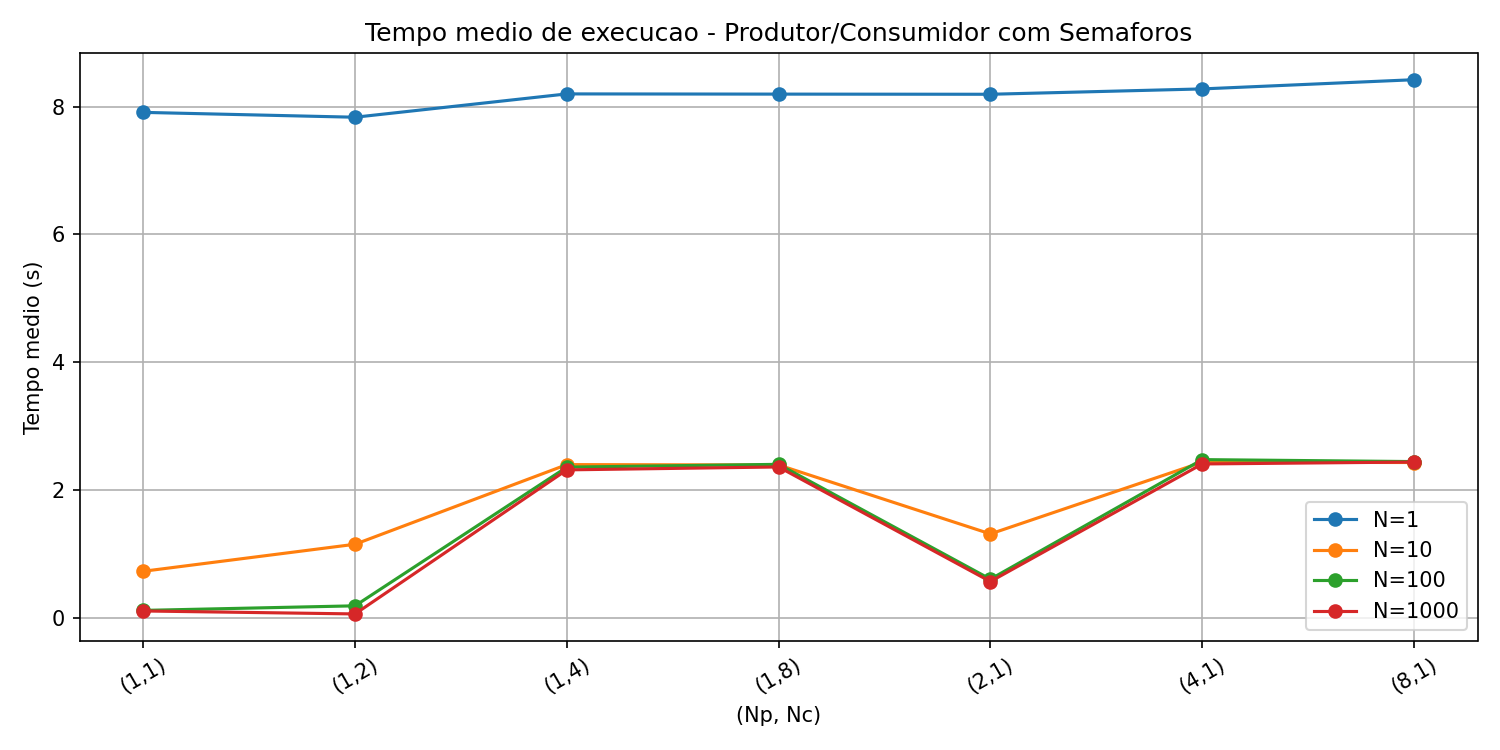
\includegraphics[width=0.92\linewidth]{tempo_medio.png}
    \caption{Tempo médio de execução em função de $(N_p, N_c)$ para cada
             tamanho de buffer $N$.}
    \label{fig:tempo}
\end{figure}

\paragraph{Análise dos tempos.}
Para $N = 1$ o buffer age como um rendezvous: produtor e consumidor
alternam-se obrigatoriamente em cada slot, resultando em $\approx 8$~s
independentemente do número de threads, adicionar threads só aumenta
a contenção no mutex sem ganho algum de paralelismo.

Para $N \geq 10$ o comportamento muda drasticamente: com $(1,1)$ e
$N = 1000$ o tempo cai para $\approx 0{,}10$~s, e com $(1,2)$ cai ainda
mais para $\approx 0{,}06$~s, pois dois consumidores paralelizam a
verificação de primalidade sem disputar excessivamente o mutex.
Contudo, a partir de 4 ou mais threads os tempos voltam a subir para
$\approx 2{,}3$–$2{,}5$~s independentemente de $N$: o overhead de
contenção no mutex e de escalonamento de threads supera o ganho de
paralelismo neste ambiente (WSL2 com núcleos limitados).

Em resumo, o ponto ótimo observado foi $(N_p, N_c) = (1,2)$ com $N = 1000$
($\approx 0{,}06$~s), enquanto o pior caso foi qualquer configuração com
$N = 1$ ($\approx 8$~s).

\begin{figure}[H]
    \centering
    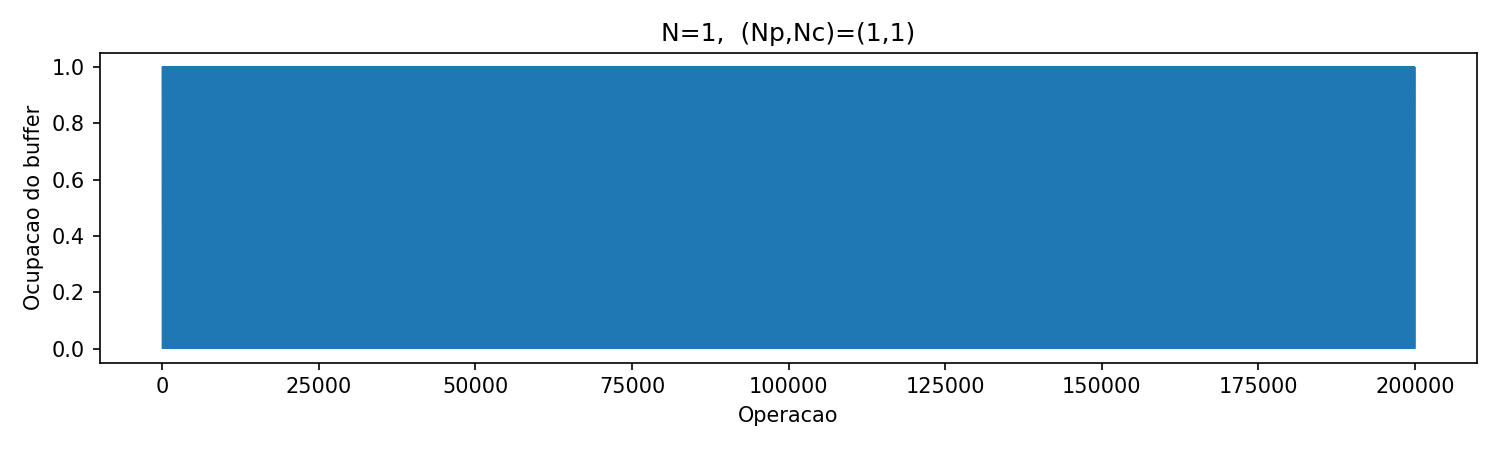
\includegraphics[width=0.48\linewidth]{occ_N1_Np1_Nc1.png}
    \hfill
    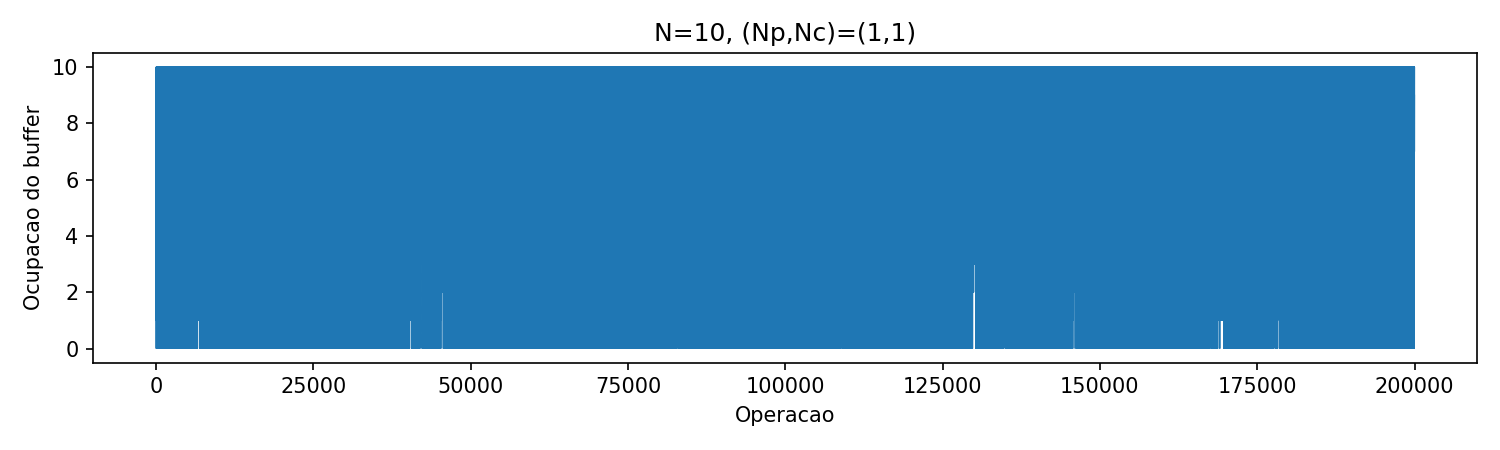
\includegraphics[width=0.48\linewidth]{occ_N10_Np1_Nc1.png}\\[4pt]
    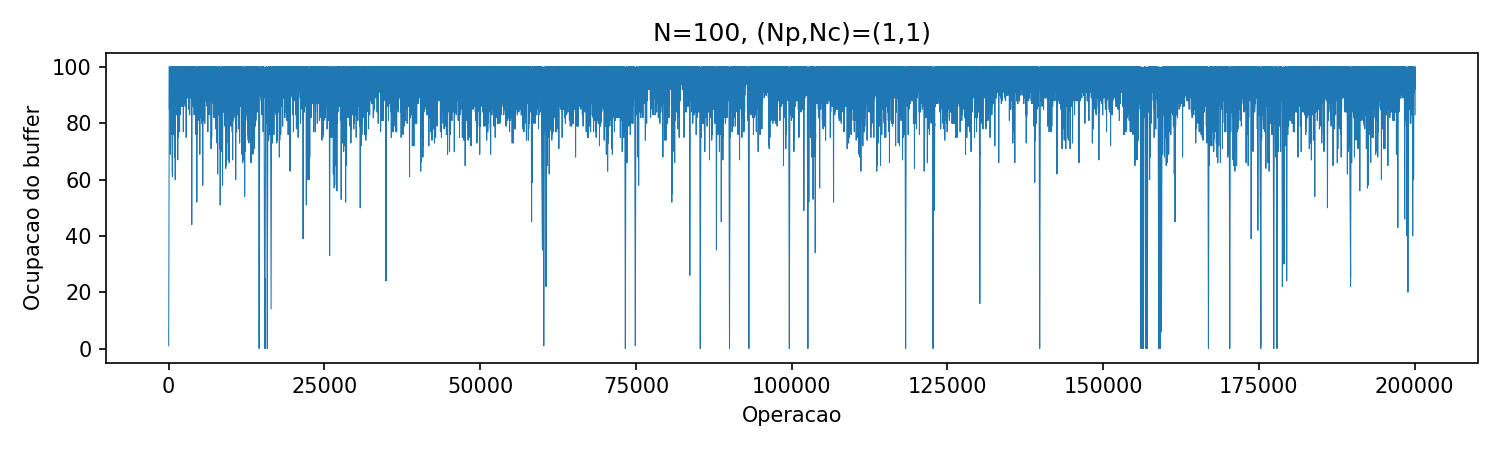
\includegraphics[width=0.48\linewidth]{occ_N100_Np1_Nc1.png}
    \hfill
    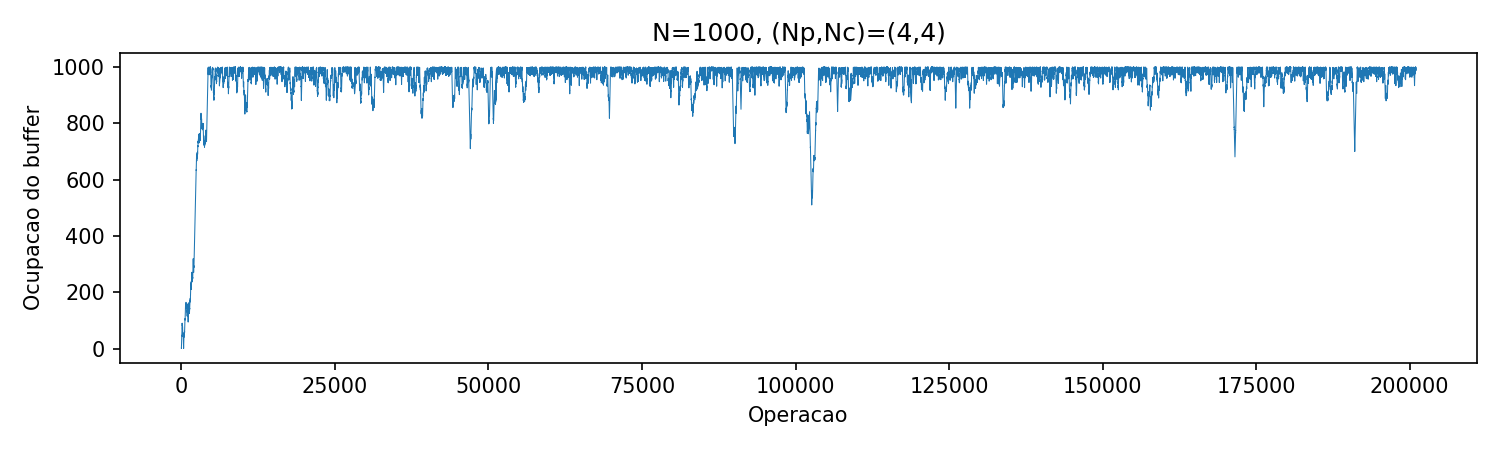
\includegraphics[width=0.48\linewidth]{occ_N1000_Np4_Nc4.png}
    \caption{Ocupação do buffer ao longo do tempo para cada valor de $N$, cenário $(N_p,N_c){=}(1,1)$
             exceto $N{=}1000$ com $(4,4)$.
             $N{=}1$: buffer alterna entre 0 e 1 (rendezvous).
             $N{=}10$: oscilações frequentes entre vazio e cheio.
             $N{=}100$: buffer se estabiliza em nível intermediário.
             $N{=}1000$: buffer enche rapidamente e permanece próximo à capacidade máxima.}
    \label{fig:occ}
\end{figure}

\paragraph{Conclusões por cenário.}
\begin{itemize}
    \item $N = 1$: buffer de tamanho 1 torna produção e consumo
          estritamente alternados (rendezvous). Mais threads apenas
          adicionam contenção; tempo $\approx 8$~s em todos os casos.
    \item $N = 10$: desempenho melhor com $(1,1)$ ($\approx 0{,}73$~s).
          Assimetria como $(1,4)$ piora para $\approx 2{,}4$~s.
    \item $N = 100$ e $N = 1000$: $(1,1)$ e $(1,2)$ são os mais rápidos
          ($\approx 0{,}06$–$0{,}11$~s). O buffer grande desacopla
          produção e consumo, e dois consumidores paralelizam a
          primalidade eficientemente.
    \item Configurações com $\geq 4$ threads: plateau de $\approx 2{,}3$~s
          em todos os valores de $N$, indicando que o gargalo passa a
          ser o escalonador e a contenção no mutex, não o tamanho do buffer.
\end{itemize}

% -------------------------------------------------------
\section{Conclusão}

O trabalho demonstrou os dois principais mecanismos de IPC estudados.
Pipes anônimos oferecem comunicação simples entre processos pai/filho com
sincronização implícita pelo kernel. Semáforos POSIX permitem coordenar
múltiplas threads sobre memória compartilhada de forma eficiente, mas
exigem cuidado com terminação (acorde de threads bloqueadas) e com
otimizações do compilador que podem eliminar código sem efeito colateral
observável.

\end{document}
